\chapter*{Prefacio}

Estos son los apuntes de clases de Teoría de números organizado por el \href{https://web.facebook.com/GEMFCUNI/}{Grupo Estudiantil de Matemática} durante los meses de enero y febrero del año 2018.

Muchas gracias al \href{http://imca.edu.pe/portal/index.php/es/}{Instituto de Matemática y Ciencias Afines} por brindarnos sus ambientes para llevar a cabo las clases.

Por favor, cualquier sugerencia o aviso de error escribir a {\href{mailto:gem@uni.edu.pe}{gem\MVAt uni.edu.pe}} o {\href{mailto:caznaranl@uni.pe}{caznaranl\MVAt uni.pe}}.

\begin{flushright}
	Carlos Aznarán
	
\end{flushright}

\begin{figure}[h]
	\begin{subfigure}[b]{.5\textwidth}
		\centering
		\captionsetup{justification=centering,margin=0.5cm}
		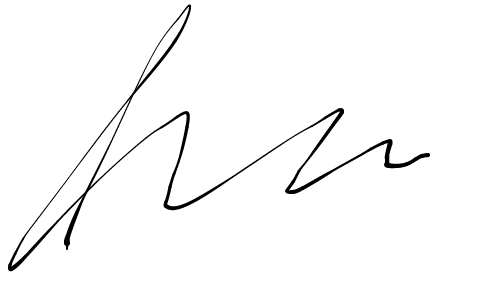
\includegraphics[height=4\baselineskip,width=.4\linewidth]{signature.png}
		\caption*{\textbf{Und. Jimmy Espinoza Palacios}\\Miembro del GEM\\Facultad de Ciencias}
	\end{subfigure}
	\begin{subfigure}[b]{.5\textwidth}
		\centering
		\captionsetup{justification=centering,margin=0.5cm}
		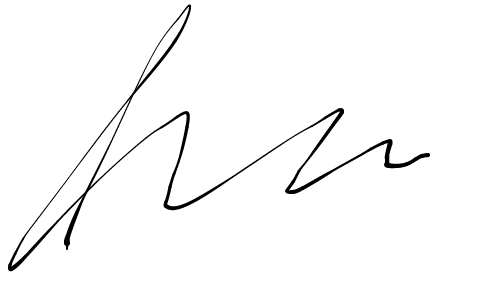
\includegraphics[height=4\baselineskip,width=.4\linewidth]{signature.png}
		\caption*{\textbf{Und. Bruno Goicochea Vilela}\\Presidente del GEM\\Facultad de Ciencias}
	\end{subfigure}
\end{figure}% Your signature
%El código fuente se puede encontrar en